%Emma Callery's Senior Seminar Paper

\documentclass{sig-alternate}
\usepackage{color}
\usepackage{listings}


\begin{document}
\conferenceinfo{UMM CSci Senior Seminar Conference, December 2014}{Morris, MN}
\title{Static and Dynamic Types in Computer Science}
\numberofauthors{1}
\author{
\alignauthor
Emma G. Callery\\
	\affaddr{Division of Science and Mathematics}\\
	\affaddr{University of Minnesota, Morris}\\
	\affaddr{Morris, Minnesota, USA 56267}\\
	\email{calle052@morris.umn.edu}
}

\maketitle

\begin{abstract}
A comparison between the benefits of static and dynamic type systems when interacting with a new or undocumented API (or other software). Specifically where in the use of the API is it beneficial to have a statically typed system over a dynamically typed system and why. 
\end{abstract}

\keywords{Static Types, Dynamic Types, Programming Languages}

\section{Introduction}
Why are we asking this question, what is a type

\section{Background Information} 
The key thing to know to answer the question posed is the difference between static types and dynamic types. Also helpful to know are the arguments made in favor and against both type systems.

\subsection{Static Types}\label{static}
In a statically typed language variables do not need to be \emph{initialized} with a value prior to use. The variable does however need to be \emph{declared} prior to use. Usually through an explicit declaration, which may include the variables initialization.  
\begin{lstlisting}
	/* C code */
	int num; // explicit declaration
	num = 5; //initialization
	int numTwo = 10; //both
\end{lstlisting}
Explicit declaration means that the variable being created is assigned a type. Thus limiting the possible values that can be assigned to the variable to be values that belong to the declared type, or a sub-type. These explicit declarations allow the type of the value to be checked against the type assigned to the variable in the declaration. This \emph{type checking} happens at compile-time; allowing type-errors, such as conflicting types, to be caught earlier. see Figure 1.  
\begin{figure}
\centering
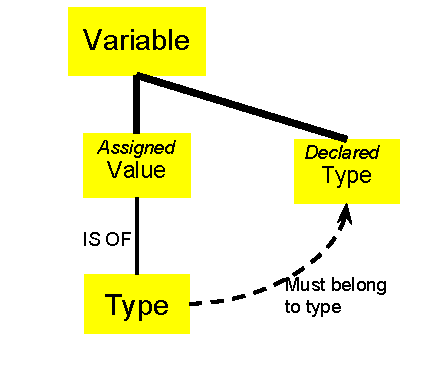
\psfig{file=Static_Type_Diagram.pdf,width =2in}
\caption{Diagram From Python Conquers the Universe of Static Types and Type Checking}
\end{figure}
\subsubsection{Arguments For Static Types}
\begin{itemize}
\item Types help to communicate to the programmer and the programmer reason about the program.
\item Requiring type names act as a form of documentation or improves the quality of the documentation.
\item Improve the programs structure.
\item Most error checking is done at compile-time, therefore catching errors more quickly.
\end{itemize}

\subsection{Dynamic Types} \label{dynamic}

A language is dynamically typed if a type is only associated with a value instead of both variables and values. see Figure 2. \begin{figure}
\centering
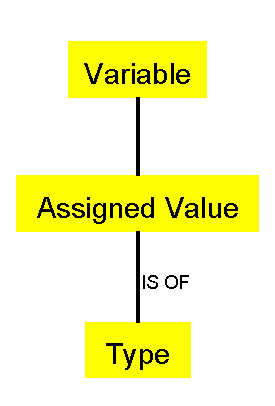
\psfig{file=Dynamic_Type_Diagram.pdf,width =1in}
\caption{Diagram From Python Conquers the Universe of Dynamic Types}
\end{figure}
This means that variables must be assigned to a value before use. 
\begin{lstlisting}
	/* Python code */
	num = 10 // direct assignment
\end{lstlisting}
This also means that there is no checking is done at compile-time, and most errors are discovered at run-time.

This does not mean that a type can not be assigned to a variable, only that the language would not require the type. This option leads to what is called \emph{optimal typing} where the programmer is primarily  responsible for the types incorporated in the program, as explained in section \ref{programmers}. 

\subsubsection{Arguments For Dynamic Types}
\begin{itemize}
\item More flexible, variables can be passed between functions more easily.
\item Without the need to declare every variable will make the program shorter, and therefore faster to write and read.
\item Programs without specific type requirements can be easily reused, with out having to write a whole new function to do the same thing to a different type
\item Not needing to declare variables, along with other 'administrative' commands, just to keep the compiler running allows for focusing to the conceptual concepts of the program.
\end{itemize}

\section{Programmer Preferences} \label{programmers}
This section will look at a study which attempted to determine where programmers use types and what types they used. The language used is the optional type language \emph{Groovy}. Groovy is a dynamically typed language that can access the static types in Java, claiming to "seamlessly integrate with existing Java classes"
\subsection{Study on Optional Typing}
Carlos Souza and Eduardo Figueiredo tried to understand programmer preferences in their paper \emph{How do Programmers Use Optional Typing? An Empirical Study}. In this study Souza and Figueiredo looked at 6638 projects written in the language Groovy. Looking over all of the projects Souza and Figueiredo tried to answer several questions about the use of types in the different projects.

\subsection{results of study on optional typing}


\section{Static V Dynamic Type Systems}

\section{Influence}

\section{Conclusions}
There are places where Dynamic is better then Static, and the surprising point where types no longer matter as much.

\section{Acknowledgments}

\section{References}
\bibliography{My_paper}  
\bibliographystyle{abbrv}

\end{document}
